\documentclass[a4paper,10pt,french]{article}

\usepackage[utf8]{inputenc}
\usepackage[T1]{fontenc} 
\usepackage{graphicx,psfrag}
\usepackage[frenchb]{babel}
\usepackage{ae,aecompl}
\usepackage{float}
\usepackage{fancyhdr}
\renewcommand{\baselinestretch}{1.2}

\graphicspath{{./}{./FIGURES/}}

%%%%%%%%%%%%%%%%%%%%%%%%%%%%%%%%%%%%%%%%%%%%%%%%%%%%%%%%%%%%

\setlength{\textwidth}{18cm}
\setlength{\textheight}{25cm}
\setlength{\oddsidemargin}{-1cm}
\setlength{\evensidemargin}{0cm}
\setlength{\topmargin}{-2cm}
\setlength{\parindent}{0cm}

%%%%%%%%%%%%%%%%%%%%%%%%%%%%%%%%%%%%%%%%%%%%%%%%%%%%%%%%%%%%
\pagestyle{fancy}

\renewcommand{\footrulewidth}{0.4 pt}
\renewcommand{\headrulewidth}{0 pt}

\newcommand{\fct}[1]{\texttt{#1}}
\newcommand{\menu}[1]{\texttt{#1}}
\newcommand{\code}[1]{\texttt{#1}}
\newcommand{\pkg}[1]{\textsf{#1}}

%%%%%%%%%%%%%%%%%%%%%%%%%%%%%%%%%%%%%%%%%%%%%%%%%%%%%%%%%%%%

\begin{document}
\thispagestyle{empty}

%\vspace*{-3cm}~\\
\hspace*{-0.5cm}

%%%%%%%%%%%%%%%%%%%%%%%%%%%% Titre %%%%%%%%%%%%%%%%%%%%%%%%%%%%%%%%%%%%
\begin{center}
\LARGE Introduction aux graphiques avec \textsf{R}
\end{center}
\bigskip

%%%%%%%%%%%%%%%%%%%%%%%%%%%%%%%%%%%%%%%%%%%%%%%%%%%%%%%%%%%%%%%%%%%%%%
\section{Trac\'e d'une fonction}
\begin{enumerate}
\item Tracer la fonction sinus entre 0 et $2\pi$ (utiliser \code{pi}).
\item Ajouter le titre (\code{\fct{title}}) suivant: \code{Graphe de la fonction sinus}.
\end{enumerate}


\section{Trac\'e de deux fonctions}
\begin{enumerate}
\item Sur une m\^eme fen\^etre graphique tracer 2 graphiques
  (\texttt{par}): la fonction $f:x\mapsto
  f(x)=\frac{1}{\sqrt{2\pi}}\exp(-0.5x^2)$ entre $-3$ et $3$ et
    la fonction $g:x\mapsto
    g(x)=\frac{1}{\sqrt{2\pi}}\exp(-0.5(x-4)^2)$ entre $1$
      et $7$.
\item Sachant que la densit\'e de la loi normale de param\`etres $\mu,\sigma^2$ est donn\'ee par $\frac{1}{\sqrt{2\pi}\sigma}\exp(-\frac{(x-\mu)^2}{2\sigma^2})$ identifier $\mu$ et $\sigma^2$ pour les deux densit\'es $f$ et $g$ ci dessus. 
\end{enumerate}


%%%%%%%%%%%%%%%%%%%%%%%%%%%%%%%%%%%%%%%%%%%%%%%%%%%%%%%%%%%%%%%%%%%%
\section{Comparaison de distributions}
\begin{enumerate}
\item Tracer la courbe de la loi normale entre -4 et 4 (utiliser \code{\fct{dnorm}}).
\item Tracer sur le m\^eme graphe les lois de Student \`a 5 et 30 degr\'es de libert\'e. Utiliser la fonction \code{\fct{curve}}
et une couleur diff\'erente pour chaque courbe.
\item Ajouter une l\'egende en haut \`a gauche pour diff\'erencier chaque distribution.
\end{enumerate}

%%%%%%%%%%%%%%%%%%%%%%%%%%%%%%%%%%%%%%%%%%%%%%%%%%%%%%%%%%%%%%%%%%%%
\section{Trac\'e de points}
\begin{enumerate}
\item Importer le tableau \code{ozone} et tracer le nuage de points du maximum d'ozone (\code{maxO3}) en
  fonction de la temp\'erature (\code{T12}).
\item Tracer le nuage de points \code{maxO3} en
  fonction de \code{T12} avec des lignes reliant les points.
\item En utilisant \code{\fct{order}} tracer le graphique \ref{fig:extracepts}.
  \begin{figure}[H]
    \centering
    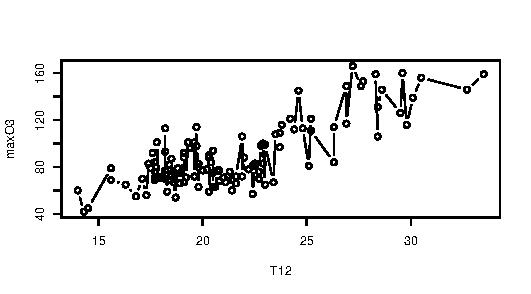
\includegraphics{graphe_base_tracepts}
    \caption{Nuage de points \code{maxO3} en
  fonction de \code{T12}.}
    \label{fig:extracepts}
  \end{figure}
\item Identifier le point ayant l'ordonn\'ee la plus \'elev\'ee (s\'election par \texttt{[]}). Identifier un point quelconque \`a la souris (voir \texttt{identify}).
\end{enumerate}


%%%%%%%%%%%%%%%%%%%%%%%%%%%%%%%%%%%%%%%%%%%%%%%%%%%%%%%%%%%%%%%%%%%%
\section{Trac\'e des taches solaires}
\begin{enumerate}
\item Importer la s\'erie \code{taches\_solaires.csv} qui donne, date par
  date, le nombre relatif de taches solaires. V\'erifier le type des
  variables \`a l'issue de l'importation.
\item Cr\'eer une variable qualitative \code{trentenaire} \'egale \`a 1 pour la premi\`ere
ann\'ee (1749) et qui augmente de 1 tous les trente ans. Pour cela, utiliser l'arrondi
(\code{\fct{floor}}) de la division par 30 (ou la division enti\`ere).
\item Saisir le vecteur \code{couleur} qui contient les couleurs suivantes: green,
  yellow, magenta, orange, cyan, grey, red, green et blue.
  V\'erifier automatiquement que ces couleurs sont bien contenues dans le vecteur \code{\fct{colors}()} (instructions \code{\%in\%} et \code{\fct{all}}).
\item Tracer la s\'erie chronologique comme dans la figure
  \ref{fig:extaches}. Utiliser les fonctions \code{\fct{palette}},
  \code{\fct{plot}}, \code{\fct{lines}} et une boucle (voir aussi
  \code{\fct{unique}}).
  \begin{figure}[H]
    \centering
    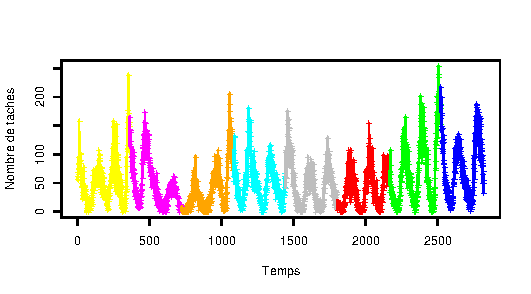
\includegraphics{graphe_base_taches}
    \caption{Taches solaires en fonction du num\'ero d'observation.}
    \label{fig:extaches}
  \end{figure}
\end{enumerate}


%%%%%%%%%%%%%%%%%%%%%%%%%%%%%%%%%%%%%%%%%%%%%%%%%%%%%%%%%%%%%%%%%%%%
\section{Affiner son graphique}
\begin{enumerate}
\item En utilisant le tableau \code{ozone} et tracer le nuage de points de la temp\'erature \`a 15h (\code{T15}) en
  fonction de la temp\'erature \`a midi (\code{T12}).
\item Obtenir le graphique suivant 
  \begin{figure}[H]
    \centering
    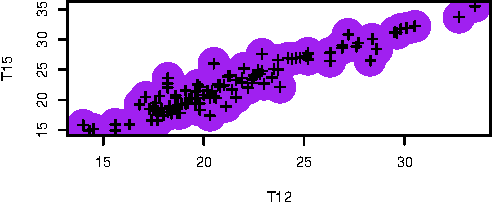
\includegraphics{pch}
    \caption{Nuage de points \code{T15} en
  fonction de \code{T12}.}
  \end{figure}
\item Obtenir le graphique suivant (voir les options \texttt{yaxt, cex.axis},  la fonction \texttt{axis} et l'argument \texttt{las}). 
  \begin{figure}[H]
    \centering
    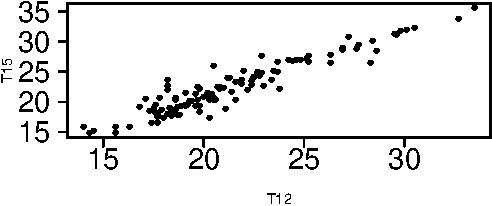
\includegraphics{axes}
    \caption{Nuage de points \code{T15} en
  fonction de \code{T12}.}
 \end{figure}
\end{enumerate}


%%%%%%%%%%%%%%%%%%%%%%%%%%%%%%%%%%%%%%%%%%%%%%%%%%%%%%%%%%%%%%%%%%%%%
\section{Trac\'e d'une densit\'e}
\begin{enumerate}
\item Tracer la densit\'e de la variable al\'eatoire $X$, $X\sim\mathcal{N}(0,1)$ (voir \code{\fct{dnorm}}).
\item Ajouter l'axe des abscisses (voir \code{\fct{abline}}).
\item Colorier en bleu l'aire sous la courbe \`a droite de $q$ correspondant \`a la probabilit\'e de 5~\% (\code{\fct{polygon}}).
\item Ajouter une fl\`eche d\'esignant l'aire colori\'ee (\code{\fct{arrows}}).
\item Indiquer au bout de la fl\`eche $\alpha=5~\%$ (\code{\fct{text}} et \code{\fct{expression}}):
  \begin{figure}[H]
    \centering
    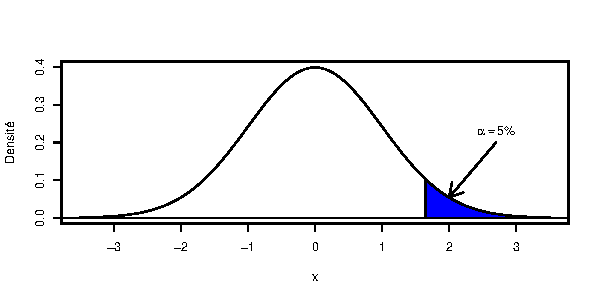
\includegraphics{graphe_base_densite}
    \caption{Densit\'e d'une loi normale.}
    \label{fig:exdensite}
  \end{figure}
\end{enumerate}


%%%%%%%%%%%%%%%%%%%%%%%%%%%%%%%%%%%%%%%%%%%%%%%%%%%%%%%%%%%%%%%%%%%%
\section{Plusieurs graphiques}
\begin{enumerate}
\item Reproduire le graphique suivant (voir l'aide de \texttt{layout})
\begin{figure}[H]
\begin{center}
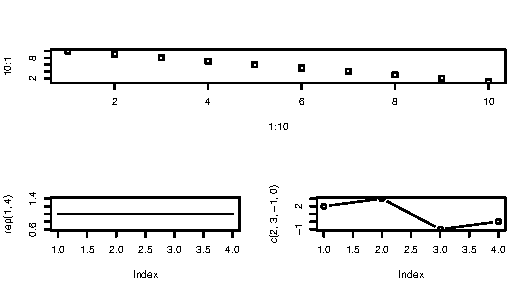
\includegraphics{layout2}
\caption{Trois graphiques sur deux lignes.\label{fig:layout3}}
\end{center}
\end{figure}
\item Reproduire le graphique suivant en jouant sur les marges (voir \texttt{par} et l'argument \texttt{mar})
\begin{figure}[H]
\begin{center}
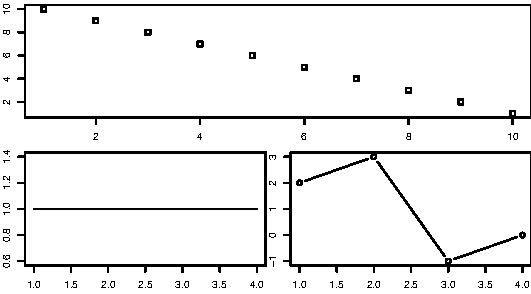
\includegraphics{layout3}
\caption{Trois graphiques sur deux lignes.\label{fig:layout3}}
\end{center}
\end{figure}
\item Reproduire le m\^eme graphique que ci-dessus mais avec un graphique en bas \`a droite d'une largeur de 1 pour 4 par rapport \`a celui en bas \`a gauche (voir les arguments de \code{\fct{layout}}).
\end{enumerate}



\end{document}